\documentclass{beamer}

\usepackage[utf8]{inputenc}
\usepackage[english,ngerman]{babel}

\usepackage[natbib=true,style=numeric,backend=biber,useprefix=true]{biblatex}
\setbeamercolor*{bibliography entry title}{fg=black}
\setbeamercolor*{bibliography entry location}{fg=black}
\setbeamercolor*{bibliography entry note}{fg=black}
\setbeamertemplate{bibliography item}{\insertbiblabel}
\renewcommand*{\bibfont}{\scriptsize}
\addbibresource{kolloquium.bib}

\usepackage{caption}
\captionsetup[figure]{labelformat=empty}

\usetheme{Malmoe}
\usecolortheme{dove}
\usefonttheme{structurebold}

\setbeamertemplate{navigation symbols}{}%remove navigation symbols
\setbeamertemplate{footline}[frame number]{}

\usepackage{pdfcomment}
\newcommand{\pdfnote}[1]{\marginnote{\pdfcomment{#1}}}

\newcommand{\backupbegin}{
    \newcounter{framenumberappendix}
    \setcounter{framenumberappendix}{\value{framenumber}}
 }
 \newcommand{\backupend}{
    \addtocounter{framenumberappendix}{-\value{framenumber}}
    \addtocounter{framenumber}{\value{framenumberappendix}} 
 }

\title[HoloLens Anwendung für Windows Mixed Reality]{Augmented Reality Anwendung für Windows Mixed Reality unter Verwendung der HoloLens zur Vermarktung von Werbeflächen}
\date[2017]{Donnerstag, 19. Oktober 2017}
\author[S. Schröder]{Sören Schröder}
\institute[Uni Koblenz]{Universität Koblenz Landau}


\begin{document}
\begin{frame}[plain]
    \maketitle
    \begin{figure}
        \centering
        \begin{minipage}{.5\textwidth}
            \centering
            \includegraphics[width=.9\linewidth]{logos/UniLogoNeu}
        \end{minipage}%
        \begin{minipage}{.5\textwidth}
            \centering
            
\includegraphics[width=.9\linewidth]{logos/brickmakers-logo}
        \end{minipage}
    \end{figure}   

    \pdfnote{Begrüßung}
    \pdfnote{Mit Namen Vorstellen}
    \pdfnote{Titel der Arbeit}
\end{frame}

\begin{frame}[shrink=25]
    \frametitle{Inhalte}
    \tableofcontents[pausesections, hideallsubsections]
    \pdfnote{Motivation}
    \pdfnote{Aufgabenstellung}
    \pdfnote{----------------------------}
    \pdfnote{Verbaute Hardware}
    \pdfnote{----------------------------}
    \pdfnote{Anwendungsszenario}
    \pdfnote{Anforderungen}
    \pdfnote{----------------------------}
\end{frame}

\section{Einleitung}
% \begin{frame}
%     \frametitle{\insertsection}
%     \begin{itemize}[<+->]
%         \item Verbreitung AR und VR
%         \item HoloLens
%     \end{itemize}


%     \pdfnote{----------------------------}
%     \pdfnote{Ein AR Gerät: HoloLens}
%     \pdfnote{Grenzt ab zu andern AR Brillen}
%     \pdfnote{Komplett aurtark}
%     \pdfnote{Rechenleistung mobiler Computer}
%     \pdfnote{Interaktion von Virtuellem mit dem Raum}

% \end{frame}

\subsection{Motiviation}
\begin{frame}
    \frametitle{\insertsubsection} 
    \pause
    \begin{figure}
        \centering
        \begin{minipage}{.49\textwidth}
            \centering
            \includegraphics[width=.9\linewidth]{images/HoloLens}
            \caption{Microsoft HoloLens~\cite{HoloLens:uH2UA4Mc}}
        \end{minipage}
        \pause
        \begin{minipage}{.49\textwidth}
            \centering
            \includegraphics[width=.9\linewidth]{images/Billboard}
            \caption{Großfläche (Plakatwand) der awk~\cite{GrossflacheStandort:2017vl}\label{fig:Billboard}}           
        \end{minipage}
    \end{figure}  
   
    \pdfnote{Verfügbarkeit gestiegen}
    \pdfnote{Oculus, Google Cardboard}
    \pdfnote{Pokémon Go, Apple AR-Kit}
    \pdfnote{--------------------------------}
    \pdfnote{HoloLens}
    \pdfnote{HMD ähnlich wie bekannte VR Headsets}
    \pdfnote{Displays transparent -> AR Brille}
    \pdfnote{Besonderheiten im vgl. Google Glass:}
    \pdfnote{Erkennung des Raums (Spatial Mapping)}
    \pdfnote{Interaktion viertueller Elemente mit Raum}
    \pdfnote{Inside out Tracking}
    \pdfnote{Erstes Gerät dieser Art}
    \pdfnote{--------------------------------}
    \pdfnote{Neue Anwendungsbereiche}
    \pdfnote{Plakatwand der awk}
    \pdfnote{Stellt Metadaten dieser zur Verfügung}
\end{frame}

% \begin{frame}
%     \frametitle{\insertsubsection}
%     \begin{figure}
%         \centering
%         \includegraphics[width=\linewidth]{images/Billboard}
%         \caption{Großfläche (Plakatwand) der awk~\cite{GrossflacheStandort:2017vl}\label{fig:Billboard}}
%     \end{figure}

%     \pdfnote{Plakatwand der awk}
%     \pdfnote{Stellt Metadaten dieser zur Verfügung}
%     \pdfnote{Usecase: HoloLens bietet Informationen für potentielle Kunden}

% \end{frame}

\subsection{Aufgabenstellung}
\begin{frame}
    \frametitle{\insertsubsection}
    \begin{itemize}[<+->]
        \item Entwicklung eine HoloLens Anwendung
        \item Anwendung zur Vermarktung von Werbeflächen
        \item Grenzen und Möglichkeiten der HoloLens        
    \end{itemize}

    \pdfnote{Enticklung einer Anwendung für die Windows Mixed Reality Plattform, im speziellen die HoloLens}
    \pdfnote{Mixed Reality Plattform erklären}
    \pdfnote{Anwendung nur für holographische Geräte (transparent)}
    \pdfnote{--------------------------------}
    \pdfnote{Anwendung zur Vermarktung von Werbeflächen}
    \pdfnote{Anzeige der Informationen am Standort}
    \pdfnote{--------------------------------}
    \pdfnote{Forschungsfrage: Grenzen und Möglichkeiten}    
\end{frame}

% \section{Grundlagen}
% \begin{frame}
    
% \end{frame}

% \subsection{Reality-Virtuality-Conitnuum}
% \begin{frame}
%     \frametitle{\insertsubsection}  
%     \begin{figure}
%         \centering
%         \includegraphics[width=\linewidth]{images/RVC}
%         \caption{Reality-Virtuality Conitnuum nach Milgram et al. (1994)~\cite{Milgram:1994vl}}
%     \end{figure}
% \end{frame}

% \begin{frame}
%     \frametitle{Augmented Reality}
%     \begin{figure}
%         \centering
%         \includegraphics[width=\linewidth]{images/RVC}
%         \caption{Reality-Virtuality Conitnuum nach Milgram et al. (1994)~\cite{Milgram:1994vl}}
%     \end{figure}

%     % - AR: Erweitern der Realität
%     %   - Mehr Realität als virtuelle Elemente
%     %   - Realität wird angereichert
% \end{frame}

% \begin{frame}
%     \frametitle{Augmented Reality}

%     \begin{figure}
%         \centering
%         \includegraphics[width=.6\linewidth]{images/GlassNavigation}
%         \caption{Google Glass Navigation~\cite{GoogleGlassNavigat:PyBuqepU}}
%     \end{figure}

%     % - AR: Erweitern der Realität
%     %   - Beispiel Google Glass
%     %   - Weiteres Pokémon Go
% \end{frame}

% \begin{frame}
%     \frametitle{Augmented Virtuality}  
%     \begin{figure}
%         \centering
%         \includegraphics[width=\linewidth]{images/RVC}
%         \caption{Reality-Virtuality Conitnuum nach Milgram et al. (1994)~\cite{Milgram:1994vl}}
%     \end{figure}

%     % - AV: Erweitern der Virtualität
%     %   - Mehr Virtuelles als Reales
%     %   - Virtuelle Szene wird mit realen Inhalten angereichert
% \end{frame}

% \begin{frame}
%     \frametitle{Augmented Virtuality}  
    
%     \begin{figure}
%         \centering
%         \includegraphics[width=.7\linewidth]{images/weather}
%         \caption{Aufzeichnung eines Wetterberichts~\cite{WeatherForcastCWS:vz}}
%     \end{figure}

%     % - AV: Erweitern der Virtualität
%     %   - Beispiel Wetterkarte
%     %   - RVC auch auf nicht stereoskopische Lösungen anwendbar
% \end{frame}


% \begin{frame}
%     \frametitle{Virtual Reality}  
%     \begin{figure}
%         \centering
%         \includegraphics[width=\linewidth]{images/RVC}
%         \caption{Reality-Virtuality Conitnuum nach Milgram et al. (1994)~\cite{Milgram:1994vl}}
%     \end{figure}

%     % - VR: Virtuelle Realität
%     %   - Beispiel Oculus
%     %   - Unterschied zwischen VR und virtueller Umgebung
% \end{frame}

% \begin{frame}
%     \frametitle{Mixed Reality}  
%     \begin{figure}
%         \centering
%         \includegraphics[width=\linewidth]{images/RVC}
%         \caption{Reality-Virtuality Conitnuum nach Milgram et al. (1994)~\cite{Milgram:1994vl}}
%     \end{figure}

%     % - MR: Mixed Reality
%     %   - Gseamtbereich des RVC
%     %   - Übergänge zwischen den einzelnen Definitionen sind fließend Reality -> AR -> AV -> VR -> Virtuality (Matrix)
% \end{frame}

% \subsection{Mixed Reality Plattform}
% \begin{frame}
%     \frametitle{Mixed Reality Plattform}  
%     \begin{figure}
%         \centering
%         \includegraphics[width=\linewidth]{images/RVC}
%     \end{figure}

%     \begin{figure}
%         \centering
%         \begin{minipage}{.5\textwidth}
%             \centering
%             \includegraphics[width=.9\linewidth]{images/HoloLens}
%             \caption{Holographisches Gerät~\cite{HoloLens:uH2UA4Mc}}
%         \end{minipage}%
%         \begin{minipage}{.5\textwidth}
%             \centering
%             \includegraphics[width=.9\linewidth]{images/AcerMixedReality}
%             \caption{Immersives Gerät~\cite{AcerWindowsMixedR:mJmOAe22}}
%         \end{minipage}
%     \end{figure} 

%     % - Plattform von Microsoft zur Vermischung der physikalischen mit virtuellen Welten
% \end{frame}

% \begin{frame}
%     \frametitle{Mixed Reality Plattform}  

%     % - Plattform von Microsoft zur Vermischung der physikalischen mit virtuellen Welten
%     % - Zwei Geräteklassen
%     %   - Holographische Geräte (transparente Displays)
%     %   - Immersive Geräte  (opake Displays)
% \end{frame}

% \section{Microsoft HoloLens}

% \begin{frame}
%     \frametitle{\insertsection}
%     \begin{figure}
%         \centering
%             \includegraphics[width=.9\linewidth]{images/HoloLens}
%             \caption{Microsoft HoloLens~\cite{HoloLens:uH2UA4Mc}}
%       \end{figure}

%       \pdfnote{HMD ähnlich wie bekannte VR Headsets}
%       \pdfnote{Displays transparent}
%       \pdfnote{Somit kein VR sondern eher AR Gerät}
%       \pdfnote{Besonderheiten:}
%       \pdfnote{Erkennung des Raums (Spatial Mapping)}
%       \pdfnote{Interaktion viertueller Elemente mit Raum}
%       \pdfnote{Inside out Tracking}
% \end{frame}

% \begin{frame}
%     \frametitle{\insertsection}
%     \begin{figure}
%         \centering
%         \includegraphics[width=.8\linewidth]{images/HoloLensOptics.png}
%           \caption{Optik der HoloLens~\cite{Microsoft:ug}~\cite{Colaner:2016to}}
%       \end{figure}
      
%       \pdfnote{IMU: Gyroskop, Magnetometer, Beschleunigungssensor}
%       \pdfnote{Projektoren}
%       \pdfnote{Licht fällt druch optisches Gitter -> Totalreflexion}
%       \pdfnote{Fällt in Umlenkbereich und Austrittsbereich}
%       \pdfnote{Licht tritt aus -> Bild auf Display}
% \end{frame}

% \begin{frame}
%     \frametitle{\insertsection}
%     \begin{figure}
%         \centering
%         \includegraphics[width=.8\linewidth]{images/HoloLensCameras.png}
%           \caption{Sensorleiste der HoloLens~\cite{Microsoft:tn}~\cite{Colaner:2016to}}
%       \end{figure}
%       \pdfnote{Foto/Video Kamera = Webcam: Aufnahme Bilder/Videos}
%       \pdfnote{Umgebungslichtsensor}
%       \pdfnote{Tiefenkamera}
%       \pdfnote{(Time of Flieght durch Lichtpulse oder Sinusmodulation)}
%       \pdfnote{Environmental Understanding Kameras (Position im Raum)}
%       \pdfnote{Auch Gestenerkennung dabei Unterstützung Tiefenkamera}
% \end{frame}

\section{Konzeption}
\subsection{Anwendungsszenario}
\begin{frame}
    \frametitle{\insertsubsection}
    \begin{itemize}[<+->]
        \item Kunde betrachtet Plakatwände vor Ort
        \item Anwendung ermöglicht Anzeige von Informationen
    \end{itemize}
    \pdfnote{Kunde schaut Plakatwände vor Ort an}
    \pdfnote{Auswahl potentieller Werbeflächen}
    \pdfnote{----------------------------------------}
    \pdfnote{Anwendung Zeit Informationen zu Plakatwand an}
    \pdfnote{Preis, Verfügbarkeit, Kontatke pro Tag}
    \pdfnote{Benutzer kann Informationen Anfordern und wieder ausblenden}
\end{frame}

\subsection{Anforderungen}
\begin{frame}
    \frametitle{\insertsubsection}
    \begin{itemize}[<+->]
        \item Identifizierung der Plakatwand
        \item Anforderung der Informationen
        \item Anzeige der Informationen  
        \item Eindeutige Zuordnung zu Plakatwand
        \item Ausblenden der Informationen
        \item Auffindbarkeit der Informationen
        \item Aktualität der Informationen
    \end{itemize}
    \pdfnote{Identifizierung der Plakatwand}
    \pdfnote{Anforderung der Informationen}
    \pdfnote{Anzeige der Informationen}
    \pdfnote{Eindeutige Zuordnung zu Plakatwand}
    \pdfnote{Ausblenden der Informationen}
    \pdfnote{Auffindbarkeit der Informationen}
    \pdfnote{Aktualität der Informationen}
\end{frame}

\section{Lösungsanstäze}
\subsection{Identifizierung der Plakatwand}
\begin{frame}
    \frametitle{\insertsubsection}
    \begin{figure}
        \centering
        \includegraphics[width=.5\linewidth]{images/billboard_identification_1}
    \end{figure}
    
    \pdfnote{Plakatwand über Standort bestimmen}
    \pdfnote{In vielen Fällen kann dies nicht ausreichen}
    \pdfnote{Entfernung zu Plakatwand verfeinert Suche}
    \pdfnote{Tiefenkamera nur ca. 3 Meter}
    \pdfnote{Erkennung der Plakatwand mit BV: OpenCV auf HoloLens nicht möglich gewesen}
    \pdfnote{Weiter Verfeinerung über Blickrichtung: Kein Zugriff auf IMU}
\end{frame}

\subsection{Anfordern der Informationen}
\begin{frame}
    \frametitle{\insertsubsection}
    \begin{figure}
        \centering
        \includegraphics[width=\linewidth]{images/Interaction}
        \caption{Interaktion mit der HoloLens~\cite{HoloLensInteraction:IaH8RfEh}}
    \end{figure}

    \pdfnote{Eingabemethoden der HoloLens}
    \pdfnote{Gaze = Blickrichtung: Position Cursor}
    \pdfnote{Gesten: Air-Tap = Mausklick; Bloom = Windows Taste}
    \pdfnote{Sprache: Bisher nur Englisch}
    \pdfnote{In der Anwendung:}
    \pdfnote{Air-Tap fordert Informationen an}
    \pdfnote{Gaze auf Close Button und Air-Tap blendet aus}
    \pdfnote{Analog dazu Sprachbefehle}
\end{frame}

\subsection{Anzeigen der Informationen}
\begin{frame}
    \frametitle{\insertsubsection}
    \begin{figure}
        \centering
        \includegraphics[width=.6\linewidth]{images/DetailWindowInUnity}
    \end{figure}

    \pdfnote{Informationen in Fenster}
    \pdfnote{Besitzt Button zum Schließen}
    \pdfnote{Tagalong -> kein unangenehmes Gefühl wie HUD}
    \pdfnote{Billboard}
\end{frame}

\subsection{Eindeutige Zuordnung}
\begin{frame}
    \frametitle{\insertsubsection}
    \begin{figure}
        \centering
        \includegraphics[width=\linewidth]{images/UIWithoutGeolocation2}
    \end{figure}

    \pdfnote{Impliziete Zuordnung über nähe}
\end{frame}

\subsection{Aktualität der Informationen}
\begin{frame}
    \frametitle{\insertsubsection}
    \begin{itemize}[<+->]
        \item Häufige Aktualisierung der Daten
        \item Updates zu langwierig
        \item Web API
        \item Liefert Informationen zu Plakatwänden zurück
        \item Daten könne aktuell gehalten werden
    \end{itemize}

\end{frame}

\section{Struktur der Anwendung}
\begin{frame}
    \frametitle{\insertsection}
    \begin{figure}
        \centering
        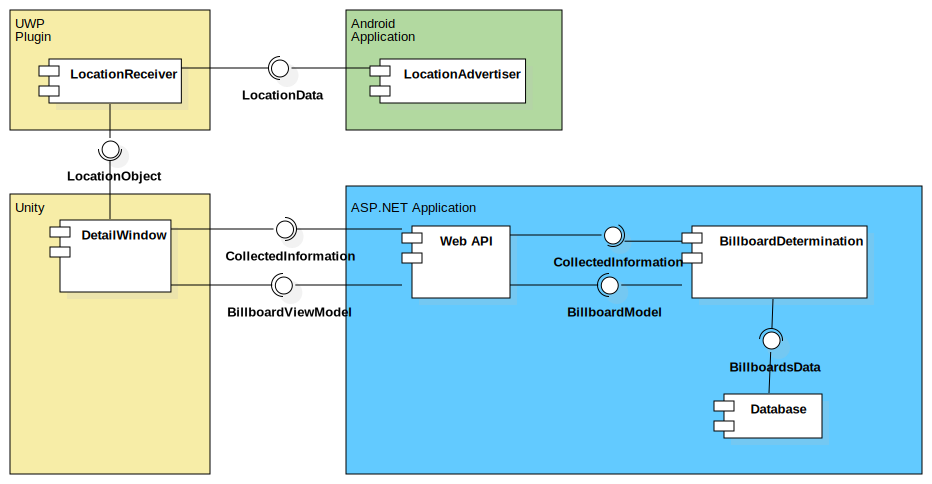
\includegraphics[width=\linewidth]{images/Komponenten}
    \end{figure}

    \pdfnote{Farben erklären}
    \pdfnote{Exemplarischer}
    \pdfnote{Web API läuft auf Server}
    \pdfnote{HoloLens und Android Anwendung Starten}
    \pdfnote{Übergabe GPS Daten erklären}
    \pdfnote{User Flow erklären}
\end{frame}

\section{Auswertung}
\subsection{Anforderungserfüllung}
\begin{frame}
    \frametitle{\insertsubsection}
    \begin{itemize}[<+->]
        \item Identifizierung der Plakatwand
        \item Anforderung der Informationen
        \item Anzeige der Informationen  
        \item Eindeutige Zuordnung zu Plakatwand
        \item Ausblenden der Informationen
        \item Auffindbarkeit der Informationen
        \item Aktualität der Informationen
    \end{itemize}

    \pdfnote{Nur für nächste Plakatwand möglich}
    \pdfnote{Flasche Ergebnisse Möglich}
    \pdfnote{----------------------------------}
    \pdfnote{Sprache und Geste}
    \pdfnote{Sprache in Lauter Umgebung möglich}
    \pdfnote{Sprache z.Z. Englisch}
    \pdfnote{----------------------------------}
    \pdfnote{Informationen werden Angzeigt}    
    \pdfnote{Sonnenschein}
    \pdfnote{----------------------------------}
    \pdfnote{Close Button}
    \pdfnote{----------------------------------}
    \pdfnote{Tagealong, Billboard}
    \pdfnote{----------------------------------}
    \pdfnote{Daten aktualisierbar}
    \pdfnote{Änderungen praktisch Zeitlich verfügbar}

\end{frame}

\subsection{Forschungsfrage}
\begin{frame}
    \frametitle{Möglichkeiten}
    \begin{itemize}[<+->]
        \item Leichter einstieg mit Unity
        \item Neue Geräteklasse
        \item Immersion
        \item Erweiterbarkeit
    \end{itemize}

    \pdfnote{Leichter Einstieg mit Unity}
    \pdfnote{Mixed Reality Toolkit}
    \pdfnote{-> Viele Entwickler Probieren aus}
    \pdfnote{---------------------------}
    \pdfnote{Neue Anwendungsfelder}
    \pdfnote{Neue Konzepte zur Beidung und Anzeige zu erforschen}
    \pdfnote{---------------------------}
    \pdfnote{Erkennung des Raums}  
    \pdfnote{---------------------------}
    \pdfnote{Einschränkungen ausgleichen}
    \pdfnote{WiFi: Daten auslager, Cloud Computing}    
    \pdfnote{Bluetooth: GPS}
\end{frame}

\begin{frame}
    \frametitle{Grenzen}
    \begin{itemize}[<+->]
        \item Entwicklungsgeschwindigkeit
        \item OpenCV
        \item Sichtfeld
        \item Akkulaufzeit
        \item Einsatz im Freien
    \end{itemize}

    \pdfnote{Häufige Build und Deployment Probleme}
    \pdfnote{teilweise Sporadisch, nicht reproduzierbar}
    \pdfnote{Lange Entwicklungkette (Viele Tools)}
    \pdfnote{------------------------------------}
    \pdfnote{OpenCV konnte nicht verwendet werden}
    \pdfnote{DLL konnte nicht geladen werden}
    \pdfnote{Lösung: Kauf des Plugins o. weiter forschen}
    \pdfnote{------------------------------------}
    \pdfnote{30° auf 17,5° (Oculus 100° auf 100°)}
    \pdfnote{Objekte am Rand nicht wirklich am Rand}
    \pdfnote{Kleineres Sichtfeld -> Weniger Informationen}
    \pdfnote{------------------------------------}
    \pdfnote{5,5 h normale Nutzung}
    \pdfnote{Bei längern Außeneinsätzen ggf. zu wenig}
    \pdfnote{Dauerhafte Wifi/Bluetooth nutzung kann veringern}
    \pdfnote{Hohe Helligkeit draußen negativ}
    \pdfnote{------------------------------------}
    \pdfnote{Display nicht ausreichend bei Sonnenschein}    
    \pdfnote{GPS umständlich}
    \pdfnote{Kein mobiles Internet -> Smartphone notwenidg}
    \pdfnote{Problem: Große Datenmengen}
\end{frame}

\section{Fazit}
\begin{frame}
    \frametitle{\insertsection}
    \begin{itemize}[<+->]
        \item Interessant
        \item Leichter Einstieg
        \item Unerwartete Probleme
        \item Erweiterung möglich
        \item Gerät für drinnen
        \item Proof of Concept
    \end{itemize}

    \pdfnote{Interssant durch neue Möglichkeiten}
    \pdfnote{Informationen präsentieren}
    \pdfnote{Nutzerinteraktion}
    \pdfnote{-----------------------------------}
    \pdfnote{Leichter Einstieg mittels Unity Möglich}
    \pdfnote{-----------------------------------}
    \pdfnote{Aufwand schwer Abschätzbar}
    \pdfnote{Probleme häufig noch nicht Dokumentiert}
    \pdfnote{Frustrationstolleranz}
    \pdfnote{-----------------------------------}
    \pdfnote{Erweiterung Möglich}
    \pdfnote{Kann teilweise schwächen draußen Ausgleich}
    \pdfnote{-----------------------------------}
    \pdfnote{Display zu Dunkel}
    \pdfnote{Akkulaufzeit begrenzt}
    \pdfnote{Möglichkeiten des Spatial Mappings drinn besser nutzbar}
    \pdfnote{-----------------------------------}
    \pdfnote{Kein fertiges Produkt eher Proof of Concept}
    \pdfnote{Hardware und Softwareseite Defizite}
    \pdfnote{Viele Komponenten erhöhen Anfälligkeit für Fehler}
\end{frame}

\section{Ausblick}

\begin{frame}
    \frametitle{\insertsection}
    \begin{itemize}[<+->]
        \item Nächste Generation der HoloLens
        \item Identifizierung der Plakatwände
        \item Verbesserung der Anzeige
        \item Überblenden von Motiven
    \end{itemize}

    \pdfnote{AI-Chip}
    \pdfnote{Erkennung von Plakatwänden}
    \pdfnote{Besser Displays}
    \pdfnote{Evtl. für drauße ausgelegt}
    \pdfnote{Unwahrscheinlich da Ökosystem für drinnen ausgelegt}
    \pdfnote{--------------------------}
    \pdfnote{Abstand zu Plakatwand}
    \pdfnote{Mit BV in OpenCV möglich}
    \pdfnote{Besser Tiefenkamera}
    \pdfnote{Daten Megentometer}
    \pdfnote{--------------------------}
    \pdfnote{Indikatoren an Plakatwand}
    \pdfnote{Standort der PW nicht bekannt}
    \pdfnote{--------------------------}
    \pdfnote{Mehrwert, da Kunde Werbung vor Druck sehen kann}
\end{frame}

\begin{frame}
    \frametitle{Fragen und Diskussion}
    Danke für Ihre Aufmerksamkeit!

    Die Folien sind unter github.com/deichcode/BachelorKolloquium zu finden.
\end{frame}

\appendix
\backupbegin{}

\begin{frame}[allowframebreaks]
    \frametitle{Quellen}
    \printbibliography{}    
\end{frame}

\section{Zusatzfolien}

\begin{frame}
    \frametitle{Reality-Virtuality-Conitnuum}  
    \begin{figure}
        \centering
        \includegraphics[width=\linewidth]{images/RVC}
        \caption{Reality-Virtuality Conitnuum nach Milgram et al. (1994)~\cite{Milgram:1994vl}}
    \end{figure}
\end{frame}

\begin{frame}
    \frametitle{Identifizierung der Plakatwand}
    \begin{figure}
        \centering
        \begin{minipage}{.5\textwidth}
            \centering
            \includegraphics[width=.9\linewidth]{images/billboard_identification_1}
        \end{minipage}%
        \begin{minipage}{.5\textwidth}
            \centering
            \includegraphics[width=.9\linewidth]{images/billboard_identification_2}
        \end{minipage}
    \end{figure}  
\end{frame}

\begin{frame}
    \frametitle{Identifizierung der Plakatwand}
    \begin{figure}
        \centering
        \begin{minipage}{.5\linewidth}
            \centering
            \includegraphics[width=.9\linewidth]{images/billboard_identification_3}
        \end{minipage}%
        \begin{minipage}{.5\linewidth}
            \centering
            \includegraphics[width=.9\linewidth]{images/billboard_identification_4}       
        \end{minipage}
    \end{figure} 
\end{frame}

\begin{frame}
    \frametitle{HoloLens Optik}
    \begin{figure}
        \centering
        \includegraphics[width=.8\linewidth]{images/HoloLensOptics.png}
          \caption{Optik der HoloLens~\cite{Microsoft:ug}~\cite{Colaner:2016to}}
      \end{figure}
      
      \pdfnote{IMU: Gyroskop, Magnetometer, Beschleunigungssensor}
      \pdfnote{Projektoren}
      \pdfnote{Licht fällt druch optisches Gitter -> Totalreflexion}
      \pdfnote{Fällt in Umlenkbereich und Austrittsbereich}
      \pdfnote{Licht tritt aus -> Bild auf Display}
\end{frame}

\begin{frame}
    \frametitle{HoloLens Sensorleiste}
    \begin{figure}
        \centering
        \includegraphics[width=.8\linewidth]{images/HoloLensCameras.png}
          \caption{Sensorleiste der HoloLens~\cite{Microsoft:tn}~\cite{Colaner:2016to}}
      \end{figure}
      \pdfnote{Foto/Video Kamera = Webcam: Aufnahme Bilder/Videos}
      \pdfnote{Umgebungslichtsensor}
      \pdfnote{Tiefenkamera}
      \pdfnote{(Time of Flieght durch Lichtpulse oder Sinusmodulation)}
      \pdfnote{Environmental Understanding Kameras (Position im Raum)}
      \pdfnote{Auch Gestenerkennung dabei Unterstützung Tiefenkamera}
\end{frame}

\backupend{}

\end{document}